\begin{figure}[!h]
    \centering
    
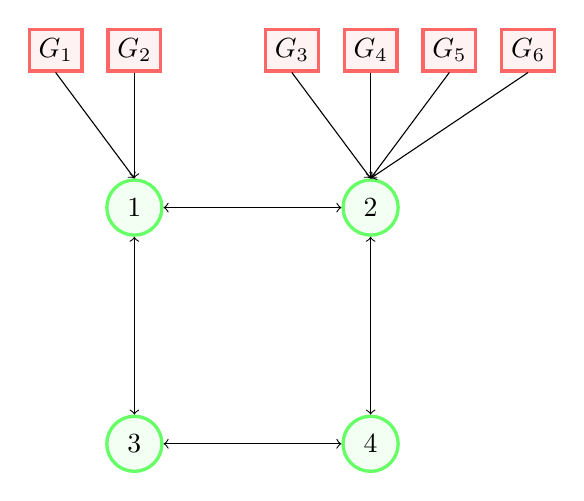
\begin{tikzpicture}[
roundnode/.style={circle, draw=green!60, fill=green!5, very thick, minimum size=7mm},
squarednode/.style={rectangle, draw=red!60, fill=red!5, very thick, minimum size=5mm},
]
%Nodes
\node[roundnode]    (node1)      at (0,0) {1};
\node[roundnode]    (node2)      at (3,0) {2};
\node[roundnode]    (node3)      at (0,-3) {3};
\node[roundnode]    (node4)      at (3,-3) {4};
\node[squarednode]  (gen1)       at (-1,2) {$G_1$};
\node[squarednode]  (gen2)       at (0,2) {$G_2$};
\node[squarednode]  (gen3)       at (2,2) {$G_3$};
\node[squarednode]  (gen4)       at (3,2) {$G_4$};
\node[squarednode]  (gen5)       at (4,2) {$G_5$};
\node[squarednode]  (gen6)       at (5,2) {$G_6$};
 
%Lines
\draw[<->] (node1.east) -- (node2.west);
\draw[<->] (node3.east) -- (node4.west);
\draw[<->] (node1.south) -- (node3.north);
\draw[<->] (node2.south) -- (node4.north);
\draw[->] (gen1.south) -- (node1.north);
\draw[->] (gen2.south) -- (node1.north);
\draw[->] (gen3.south) -- (node2.north);
\draw[->] (gen4.south) -- (node2.north);
\draw[->] (gen5.south) -- (node2.north);
\draw[->] (gen6.south) -- (node2.north);
%\draw[->] (node2.south) .. controls +(down:7mm) and +(right:7mm) .. (node3.east);
\end{tikzpicture}    
    
    \caption{Illustration of power transmission system}
    \label{fig:my_label}
\end{figure}
